\section{Container Attack Surface Analysis}
\label{sec:container-attack-surface-analysis}

In containerized environments, security challenges often arise from vulnerabilities within specific components of the architecture. As such, understanding the relationships between the different components, such as container registries, images, runtime, namespaces, cgroups, and various security modules like eBPF, seccomp, and Linux capabilities is crucial for identifying potential attack surfaces. This is where a comprehensive architecture diagram comes into play.

\begin{figure}[t]
  \label{fig:architecture}
  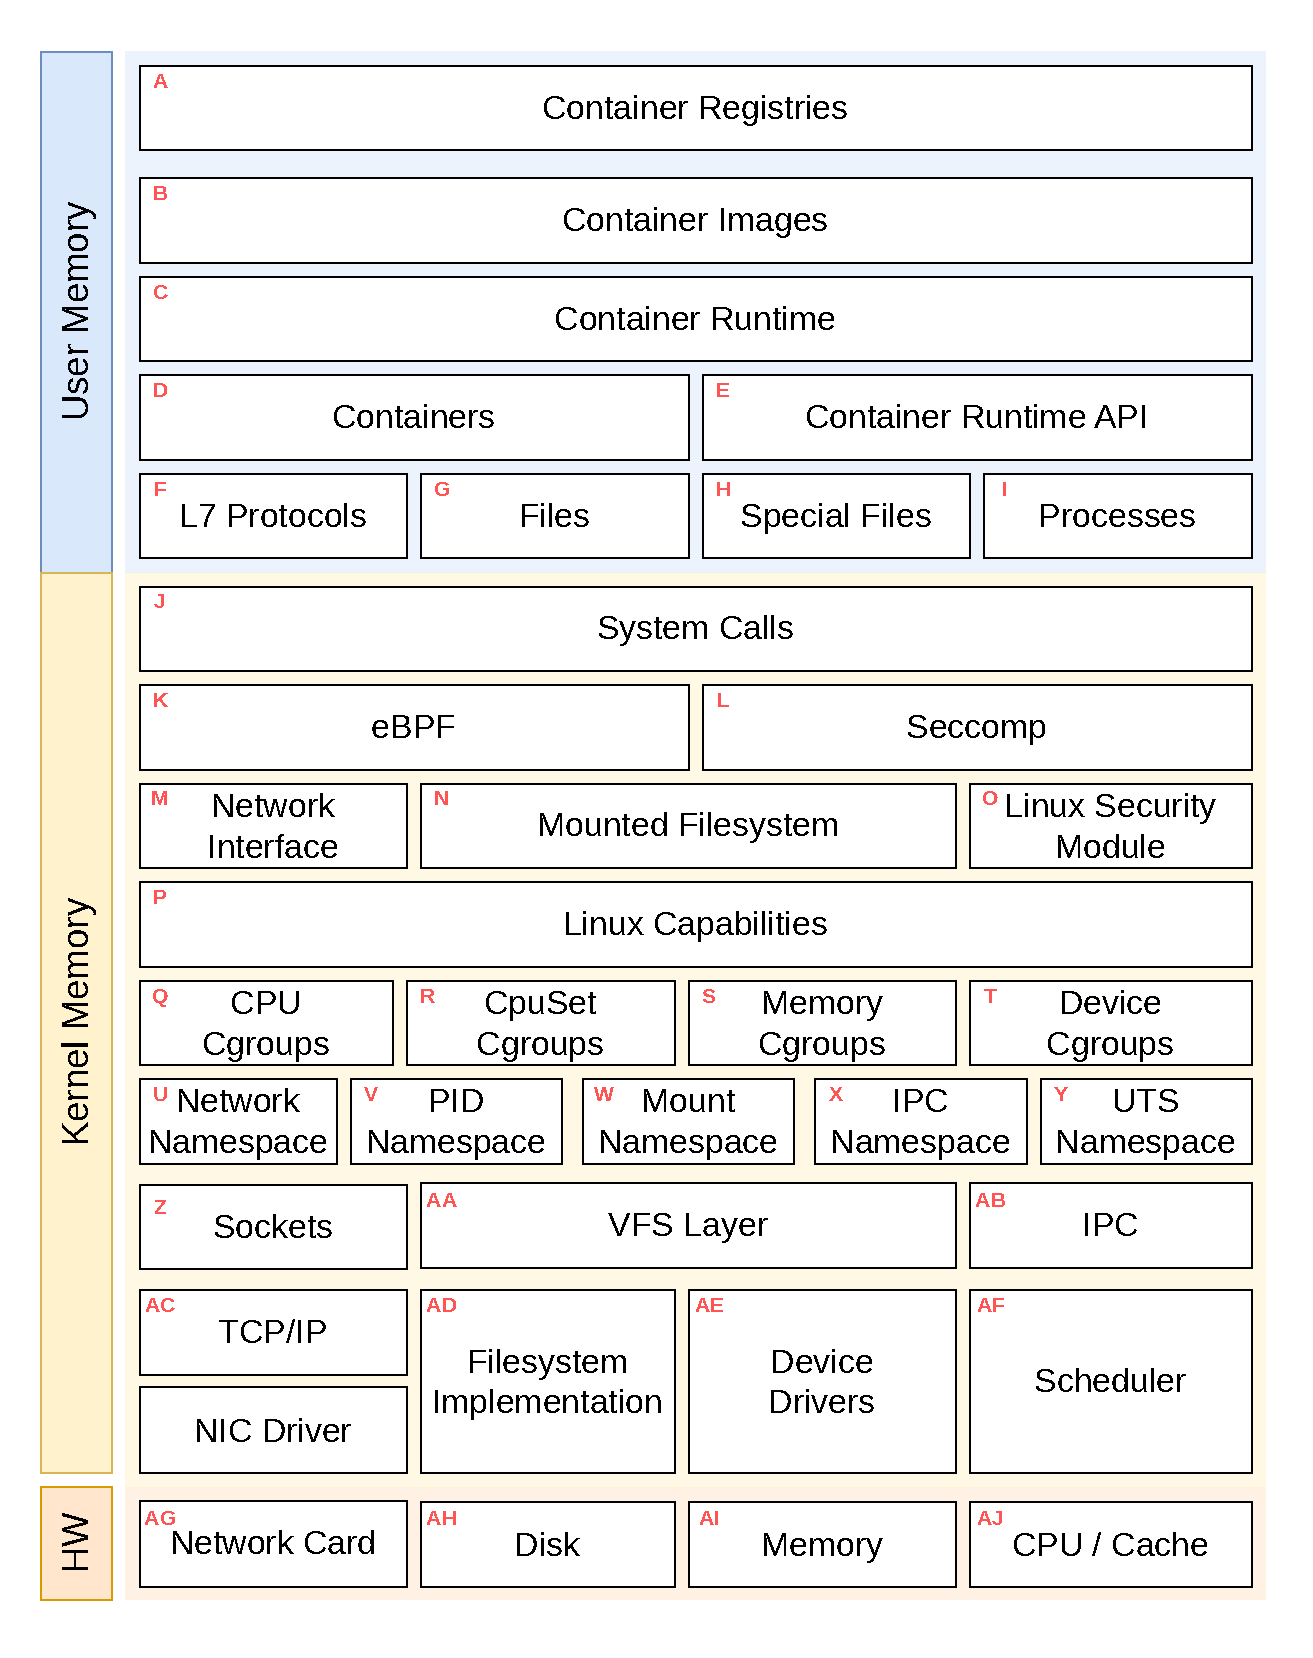
\includegraphics[width=1\linewidth]{figs/exploit-coverage.pdf}
  \caption{An architectural diagram of a container deployment environment depicting the attack surface created by its various components.}
\end{figure}

Figure 2 outlines the key components of a containerized system, highlighting the critical paths and interactions that security tests should focus on. Security testing should aim to cover these components extensively to ensure that vulnerabilities in any of these layers are adequately addressed. However, some components, like network interfaces, system calls, and cgroups, are more frequently targeted in real-world attacks and thus warrant more attention in testing. The diagram will guide our understanding of which components to prioritize during testing, ensuring that our coverage is both thorough and effective.


\section{Evaluation}
\label{sec:evaluation}

To assess the effectiveness of container confinement mechanisms, we conducted a series of controlled experiments to evaluate whether common security policies successfully prevent resource starvation, unauthorized access attempts, and container escapes. Our evaluation focuses on testing various isolation features, including namespaces, cgroups, seccomp, and Linux capabilities, under different configurations and attack scenarios. These are done in the form of three case studies.

\subsection{Case Study 1 - Evaluating Host Process Manipulation via PID Namespace Escape}

\subsubsection{Introduction to the Evaluation}

In this evaluation, we investigate whether a Docker container running with \texttt{--pid=host} can interact with and manipulate host processes. The PID namespace is responsible for process isolation, ensuring that containerized processes remain separate from host processes. However, when \texttt{--pid=host} is enabled, the container shares the host's PID namespace, making all host processes visible inside the container. We assess the security implications of this setting by evaluating the following:

\begin{dgenum}
    \item Whether a container with \texttt{--pid=host} can list host processes.
    \item Whether the container can send signals \texttt{SIGKILL}, \texttt{SIG\-TERM} to host processes.
    \item Whether enabling \texttt{CAP\_SYS\_ADMIN} allows process tracing of host processes.
    \item Whether a container can read host process memory via \texttt{/proc/\$PID/mem}.
    \item Whether a container with \texttt{--pid=host} can manipulate processes running inside another container that also has \texttt{--pid=host}.
\end{dgenum}

\subsubsection{Experimental Setup}
The experiments were conducted using Docker running inside a QEMU VM to ensure an isolated and controlled test environment. The system specifications were as follows:

\begin{itemize}
    \item \textbf{Host Machine:} 20 Core CPU, 16GB RAM, Ubuntu 24.04
    \item \textbf{Virtual Machine:} QEMU, 4 Core CPU, 12GB RAM, No Distibution
    \item \textbf{Docker Version:} 27.0.3
    \item \textbf{Kernel Version:} Linux 6.1
    \item \textbf{Container Runtime:} \texttt{runc} 1.1.11
\end{itemize}

The container was started with various security configurations:

\begin{itemize}
    \item Default Docker container configuration (separate PID namespace)
    \item Docker container with \texttt{--pid=host}
    \item Docker container with \texttt{--pid=host} and additional capabilities \texttt{CAP\_KILL}, \texttt{CAP\_SYS\_PTRACE}
    \item Privileged Docker container with \texttt{--pid=host}
    \item Two separate containers, both with \texttt{--pid=host}, to evaluate cross-container process manipulation.
\end{itemize}

For each security configuration, different methods were tested to determine whether a process inside the container could interact with host processes or another container’s processes.

\subsubsection{Security Testing}

The evaluation began by assessing whether a container with \texttt{--pid=host} could list host processes using \texttt{ps aux}. As expected, the container displayed all host processes, confirming that sharing the host PID namespace fully exposes the host process table. Following this, we tested whether the container could send termination signals (\texttt{SIGKILL}, \texttt{SIGTERM}) to host processes using \texttt{kill -9 <PID>}. Without the \texttt{CAP\_KILL} capability, the operation was not permitted. However, enabling \texttt{CAP\_KILL} allowed process termination within the namespace's limits, and granting \texttt{--privileged} access enabled the container to kill any host process. Next, we investigated whether the container could attach a debugger to host processes via \texttt{strace -p <PID>}. Without \texttt{CAP\_SYS\_PTRACE}, the operation was denied, but enabling this capability allowed successful attachment to a host process, raising concerns about potential leakage of sensitive data through system call tracing. We then examined whether the container could read host process memory by attempting to access \texttt{/proc/<host\_pid>/mem}. With Docker’s default restrictions, the operation was denied, but when running the container with \texttt{--privileged}, the process memory could be read using \texttt{cat /proc/<host\_pid>/mem}. Finally, we tested cross-container process manipulation by launching two containers with \texttt{--pid=host}. A process running in Container A (e.g., \texttt{sleep 1000}) was visible to Container B, which was able to list and terminate it, proving that containers sharing the host PID namespace are not isolated from each other and can manipulate each other's processes. This finding underscores the risk of using \texttt{--pid=host}, as it allows one compromised container to interfere with others running on the same host.

The result was that the process inside Container A was visible to Container B, and it could be terminated using \texttt{kill -9 <PID>}, proving that containers with \texttt{--pid=host} share the same namespace and are not isolated from each other.

\subsubsection{Results and Findings}

To summarize, using \texttt{ps aux}, containers with \texttt{--pid=host} could list all host processes. Sending signals \texttt{SIGKILL`, `SIGTERM} was blocked without \texttt{CAP\_KILL}, but enabling the capability allowed termination of processes within the namespace’s limits. Debugging \texttt{strace -p <PID>} required \texttt{CAP\_SYS\_PTRACE}, and reading host memory \texttt{cat /proc/<PID>/mem} was blocked unless the container was privileged. Finally, two containers with \texttt{--pid=host} were able to list and terminate each other’s processes, demonstrating cross-container process interference. The effectiveness of different configurations in preventing host and cross-container process manipulation is also illutrated in Table~\ref{tab:pid-namespace-security}.

\FloatBarrier
\begin{table*}[h]  
    \centering
    \footnotesize  
    \setlength{\tabcolsep}{4pt}  
    \renewcommand{\arraystretch}{1.1}  
    \caption{Effectiveness of Docker Security Mechanisms Against Host Process Manipulation}  
    \label{tab:pid-namespace-security}  
    \begin{adjustbox}{max width=\textwidth}  
    \begin{tabular}{|l|c|c|c|c|c|}
        \hline
        \textbf{Security Configuration} & \textbf{List Host Processes} & \textbf{Send Signals} & \textbf{Attach Debugger} & \textbf{Read Memory} & \textbf{Cross-Container Manipulation} \\ \hline
        Default Docker (PID namespace isolation) & \xmark & \xmark & \xmark & \xmark & \xmark \\ \hline
        \texttt{--pid=host} (no extra caps) & \cmark & \xmark & \xmark & \xmark & \cmark \\ \hline
        \texttt{--pid=host} + \texttt{CAP\_KILL} & \cmark & \cmark & \xmark & \xmark & \cmark \\ \hline
        \texttt{--pid=host} + \texttt{CAP\_SYS\_PTRACE} & \cmark & \xmark & \cmark & \xmark & \cmark \\ \hline
        Privileged Container (\texttt{--pid=host} + \texttt{--privileged}) & \cmark & \cmark & \cmark & \cmark & \cmark \\ \hline
    \end{tabular}  
    \end{adjustbox}  
\end{table*}

\subsubsection{Key Takeaways}
\begin{itemize}
    \item \texttt{--pid=host} completely breaks process isolation, allowing full visibility into host and cross-container processes.
    \item Containers sharing the host PID namespace can manipulate each other’s processes.
    \item Privileged containers with \texttt{--pid=host} have unrestricted access to host process memory, debugging, and termination.
\end{itemize}










\subsection{Case Study 2 - Evaluating Docker Port Forwarding Restrictions}

\subsubsection{Introduction to the Evaluation}
In this case study, we evaluate Docker’s network isolation mechanisms to determine how well they enforce port binding restrictions. Specifically, we examine whether privileged ports (1-1024) can be bound by containerized processes, and how changes in Docker’s security model (pre- and post-20.03) have affected these restrictions.

Starting with Docker version 20.03, a significant change was introduced. Docker redefined unprivileged ports to start at 0 instead of 1024, effectively removing the need for \texttt{NET\_BIND\_SERVICE} to bind to privileged ports. This has direct security implications, as it potentially allows attackers with root access inside a container to bind services to privileged ports that should traditionally require special permissions.

Thus, we evaluate two key aspects of Docker’s security model:
\begin{itemize}
    \item \textbf{Docker $\mathbf{\leq}$ 20.03:} To bind to privileged ports, root users are to use required NET\_BIND\_SERVICE.
    \item \textbf{Docker $\mathbf{\geq}$ 20.03:} Root users can bind to privileged ports without `NET\_BIND\_SERVICE`.
\end{itemize}


\subsubsection{Experimental Setup}
The experiments were conducted in a controlled QEMU-based virtualized environment, ensuring reproducibility and isolation from external interference.

\begin{itemize}
    \item \textbf{Host Machine:} 20 Core CPU, 16GB RAM, Ubuntu 24.04
    \item \textbf{Docker Versions Tested:}  
        \begin{itemize}
            \item 19.03.14 (pre-20.03)
            \item 24.0.2 (post-20.03)
        \end{itemize}
    \item \textbf{Container Runtime:} runc 1.1.7
    \item \textbf{Containers Used:}  
        \begin{itemize}
            \item Default container (bridge network mode, no additional privileges)
            \item Container with `NET\_BIND\_SERVICE`
            \item Custom seccomp profile restricting `bind` syscall
            \item Privileged mode
        \end{itemize}
\end{itemize}

Each test involved binding an HTTP server to port 23 (a privileged port), under different security configurations.

\subsubsection{Security Testing}

\noindent\textbf{1. Port Binding Restrictions in Docker < 20.03}

\textbf{Test Procedure:}
\begin{itemize}
    \item A containerized HTTP server was started, attempting to bind to port 23.
    \item Tests were conducted under varying privilege levels:
        \begin{itemize}
            \item With and without `NET\_BIND\_SERVICE`
            \item As root vs. non-root
            \item With a seccomp profile denying the `bind` syscall
        \end{itemize}
\end{itemize}

\begin{table}[h]
    \centering
    \caption{Effectiveness of Docker Security Mechanisms in Port Binding (Docker < 20.03)}
    \label{tab:port-binding-pre-20.03}
    \small
    \begin{tabular}{|p{6cm}|c|}
        \hline
        \textbf{Security Configuration} & \textbf{Result} \\ \hline
        \texttt{NET\_BIND\_SERVICE + root} & \cmark \\ \hline
        \texttt{root} & \xmark \\ \hline
        \texttt{NET\_BIND\_SERVICE + custom Seccomp (deny bind syscall) + root} & \xmark \\ \hline
        \texttt{NET\_BIND\_SERVICE + non-root} & \xmark \\ \hline
    \end{tabular}
\end{table}

\noindent\textbf{2. Port Binding Restrictions in Docker $\geq$ 20.03}

\textbf{Test Procedure:}
\begin{itemize}
    \item The same HTTP server was used, attempting to bind to port 23.
    \item We evaluated how removing `NET\_BIND\_SERVICE` affected the ability to bind to privileged ports.
\end{itemize}

\begin{table}[h]
    \centering
    \caption{Effectiveness of Docker Security Mechanisms in Port Binding (Docker $\geq$ 20.03)}
    \label{tab:port-binding-post-20.03}
    \small
    \begin{tabular}{|p{6cm}|c|}
        \hline
        \textbf{Security Configuration} & \textbf{Result} \\ \hline
        \texttt{root} & \cmark \\ \hline
        \texttt{Custom Seccomp (deny bind syscall) + root} & \xmark \\ \hline
        \texttt{non-root} & \xmark \\ \hline
    \end{tabular}
\end{table}

\subsubsection{Key Takeaways}
\begin{itemize}
    \item \textbf{Docker < 20.03:} `NET\_BIND\_SERVICE` was required to bind to privileged ports.
    \item \textbf{Docker $\geq$ 20.03:} Root containers can bind to privileged ports without `NET\_BIND\_SERVICE`.
\end{itemize}







\section{Case Study 3: Evaluating CVE-2024-21616}

\subsection{Introduction}
CVE-2024-21616 is a critical vulnerability affecting Docker and runc that allows malicious containers to escape their isolation and execute arbitrary commands on the host system. This poses a significant risk to enterprises relying on containerization, as attackers could gain unauthorized access to sensitive data and system resources. 

The root cause of this vulnerability is the improper handling of a container’s working directory when set to a special file descriptor path such as \texttt{/proc/self/fd/<fd>}, where \texttt{<fd>} typically points to \texttt{/sys/fs/cgroup}. If exploited, this flaw allows a containerized process to break out of its confined environment, effectively compromising the host machine. The vulnerability affects runc versions from \texttt{v1.0.0-rc93} to \texttt{1.1.11}.

In this case study, we leverage Houdini to systematically assess the effectiveness of Docker’s security mechanisms in mitigating CVE-2024-21616. By integrating the vulnerability as a Houdini trick, we analyze the conditions under which the exploit succeeds and evaluate different security configurations.

\subsection{Methodology}
To test the exploitability of CVE-2024-21616, we designed a Houdini trick that executes the following steps:
\begin{enumerate}
    \item Launch a container with a vulnerable version of runc.
    \item Set the working directory to \texttt{/proc/self/fd/<fd>}, pointing to a controlled file descriptor.
    \item Attempt to break out of the container by leveraging the misconfigured working directory.
    \item Validate whether commands can be executed on the host system.
\end{enumerate}

\subsection{Experimental Setup}
We conducted tests across three different configurations:
\begin{enumerate}
    \item \textbf{Default Docker Configuration:} No additional security measures.
    \item \textbf{Hardened Configuration:} Using seccomp, AppArmor, and dropping unnecessary capabilities.
    \item \textbf{Patched Environment:} Upgrading runc to version \texttt{1.1.12} or later.
\end{enumerate}

\subsection{Results and Findings}

\begin{table}[h]
    \centering
    \caption{Effectiveness of Docker Security Configurations Against CVE-2024-21616}
    \begin{tabular}{|l|c|}
        \hline
        \textbf{Configuration} & \textbf{Exploit Success} \\
        \hline
        Default Docker (runc 1.1.11) & \cmark \\
        Hardened Security Profile (runc 1.1.11) & \cmark \\
        runc 1.1.12+ & \xmark \\
        \hline
    \end{tabular}
    \label{tab:cve_results}
\end{table}

Our findings reveal that neither Docker’s default security settings nor additional confinement mechanisms (e.g., seccomp, AppArmor) were effective in preventing exploitation. The only mitigation strategy that successfully blocked the attack was upgrading runc beyond version \texttt{1.1.11}, as the vulnerability lies within the container runtime itself.